\documentclass{article}
\usepackage[utf8]{inputenc}
\usepackage{amsmath}
%}\usepackage{natbib}
\usepackage{graphicx}

\newcommand\ha{\ensuremath{\mathrm{H}\alpha}}

\title{Bowshock en la Nebulosa de Orión}

\begin{document}
\maketitle
Acontinuación presentamos algunos imágenes de los choques de proa estacionarios (bowshocks) de los 73 objetos que hemos identificado en la Nebulosa de Orión. En este sentido estos choques presentan algunas particularidades que valdría la pena mencionar, en este orden de ideas tenemos que por ejemplo, w069-601 y LL2 (aunque en este úñtimo parece estar afectado por otros fenómenos) presenta un choque muy bien definido donde esta región es muy radiativa en \(\ha\) por tanto se pueden ver muy claramente los límites de la zona chocada, además de eso se puede ver que el choque es muy simétrico como la ilustarn los círculos ajustados a las posiciones del mismo y de la misma forma pensamos que podría tratarse de un Proplyds. Por otro lado tenemos que para 173-342 y 205-230 se forman los choques debido a la interacción de los flujo de dos estrellas jóvenes que están muy cercas, entonces estaríamos frente a choques interproplyds.\\

Ahora algo singular es que algunos de estos objetos presentan doble choques que es el caso de w005-514, LL3 y LL2, donde en las imágenes obtenidas se aprecia que se forman dos choques para un mismo objeto, hay que resaltar que la estrella central de w005-5014 es un proplyd. Si continuamos con el análisis algunos dde nuestros objetos muesstran jets, en este sentido tenemos que w044-527 tiene un jet paralelo al eje de simetría, que como se puede ver en la imagen alteran de una u otra manera la forma del choque para este objeto en partícular. Vale también la pena mencionar que 102-3039, al igual que el objeto mencionado anteriormente también presenta un choque pero con la diferencia de que este es perpendicular al eje.\\

Algunos de estos objetos tienen una emisión muy débil en \(\ha\), por tanto no se pueden ver muy bien los choques de proa y en en nuestra lista este es el caso de 102-157, en que se aprecia que la región chocada es muy débil, y muchos de nuestros objetos presentan estas particularidad y las caracterísiticas mencionadas arriba, dejando claro que la forma, los parámetros físcos y demás factores pueden variar en los mismos dependiendo a las condiciones a las que estén sometidas. 

  

. 

\begin{figure*}[htp]
\centering
\begin{tabular}{l l l}
     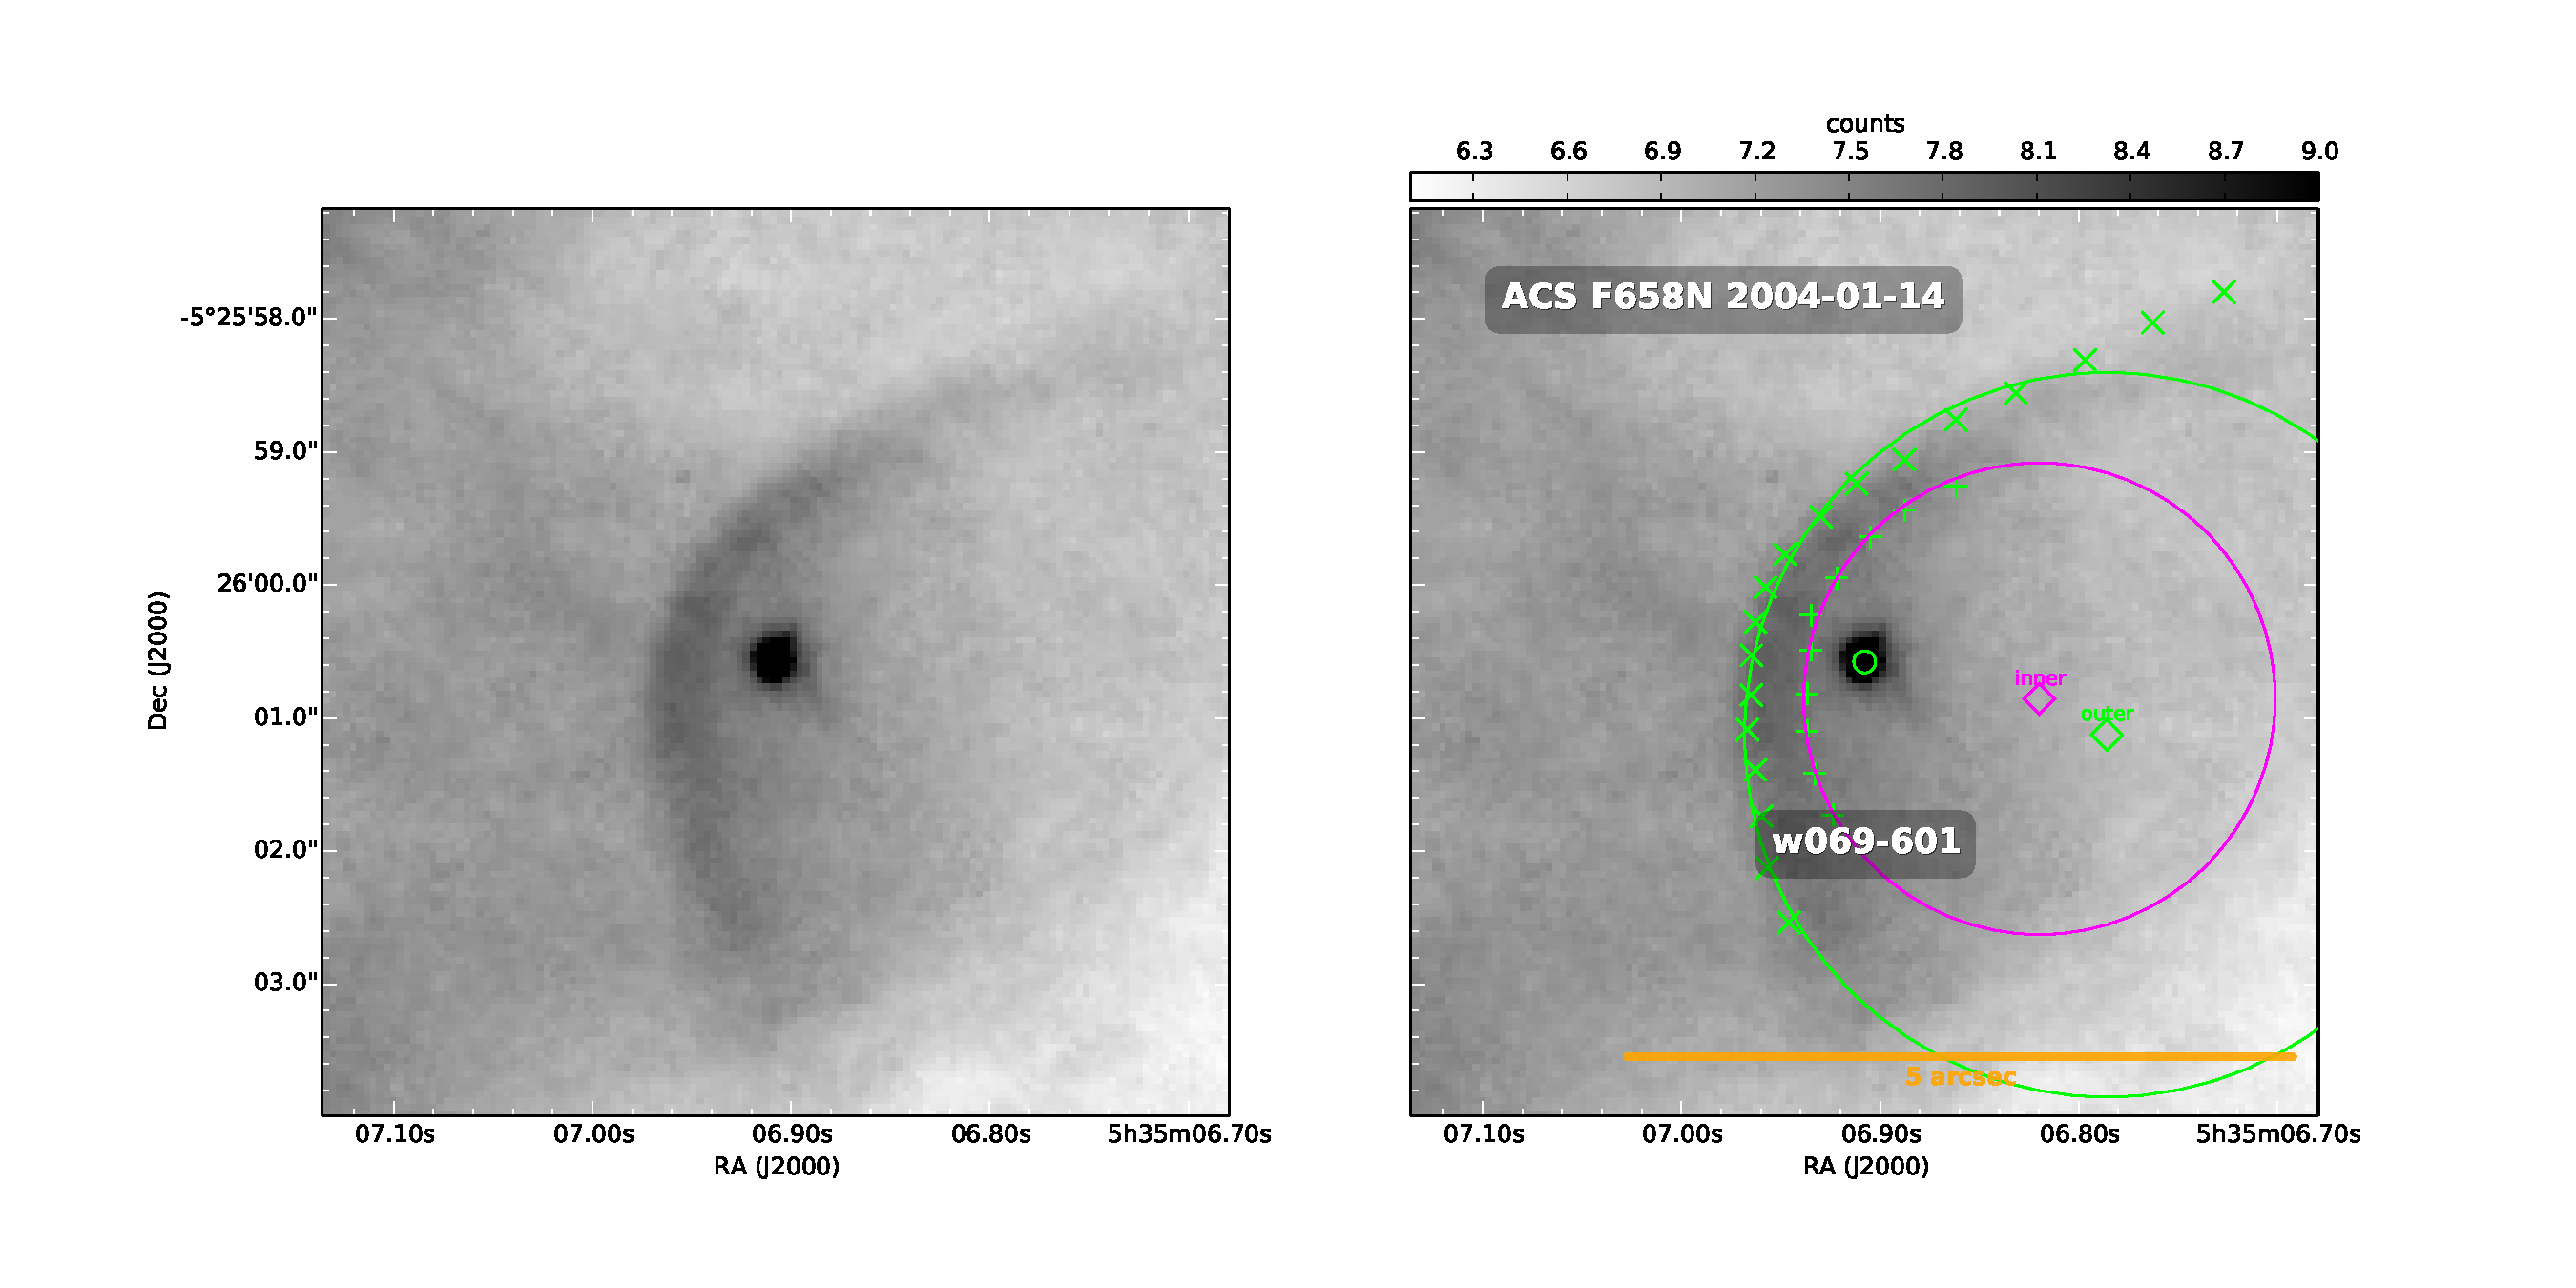
\includegraphics[width=0.5\linewidth, trim=60 50 100 50]{j8oc01010_wcs/w069-601-Bally_01-images.pdf}
    &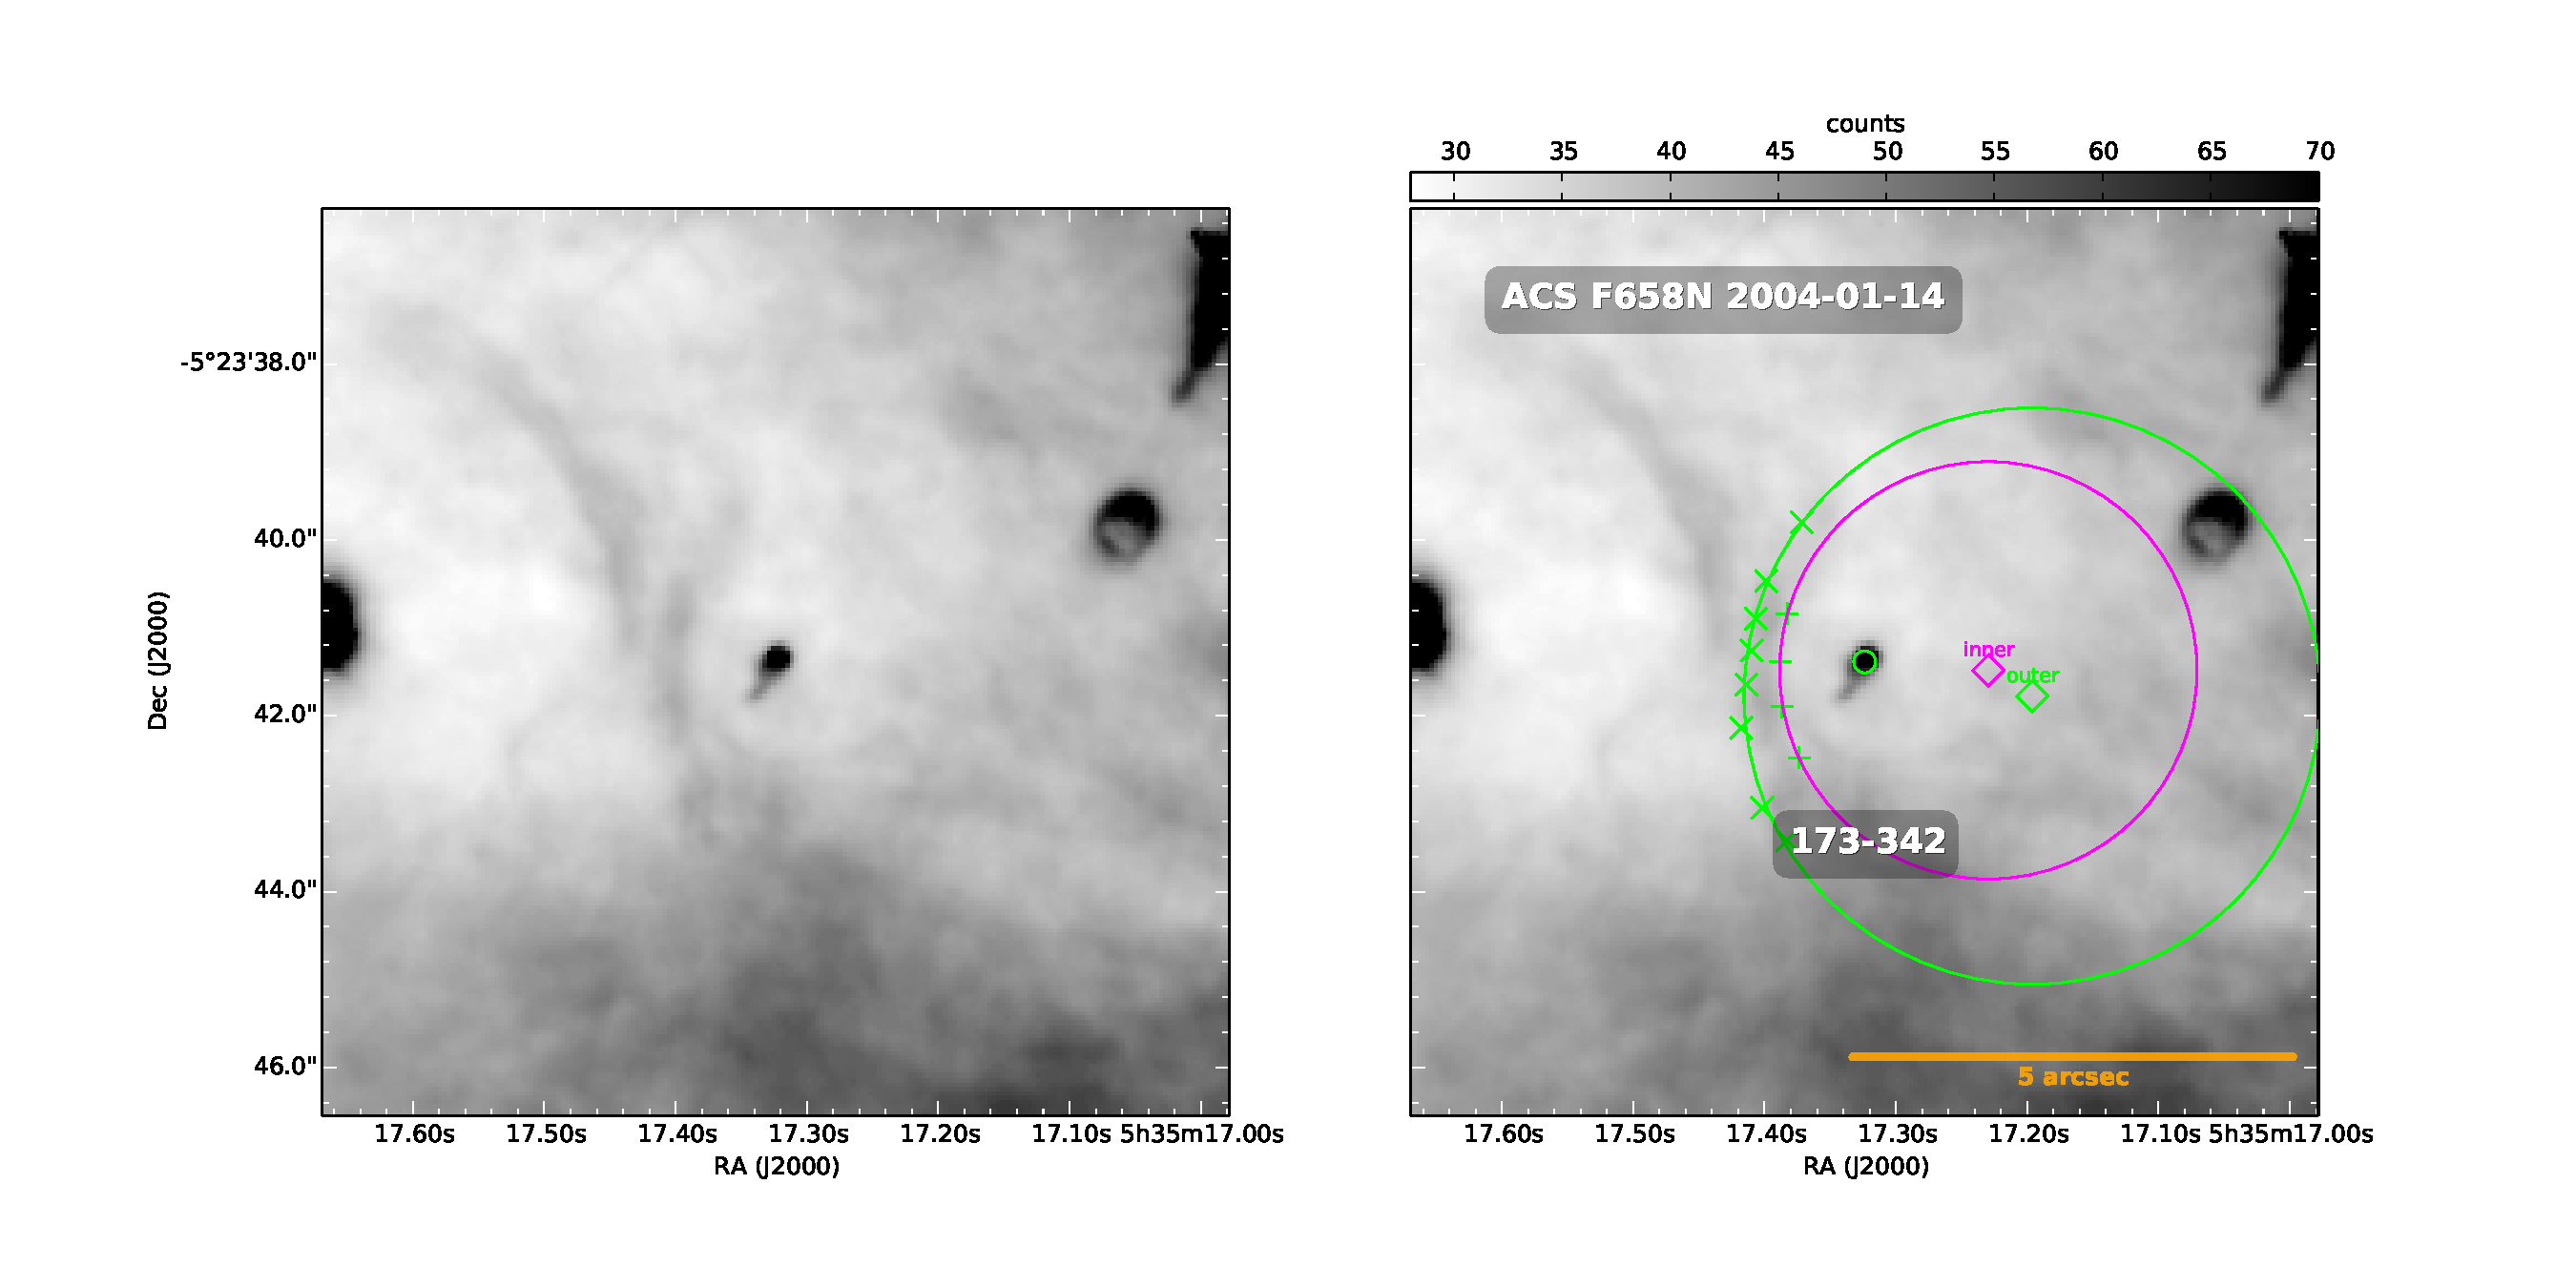
\includegraphics[width=0.5\linewidth, trim=60 50 100 50]{j8oc01010_wcs/173-342-Bally_01-images.pdf}\\
    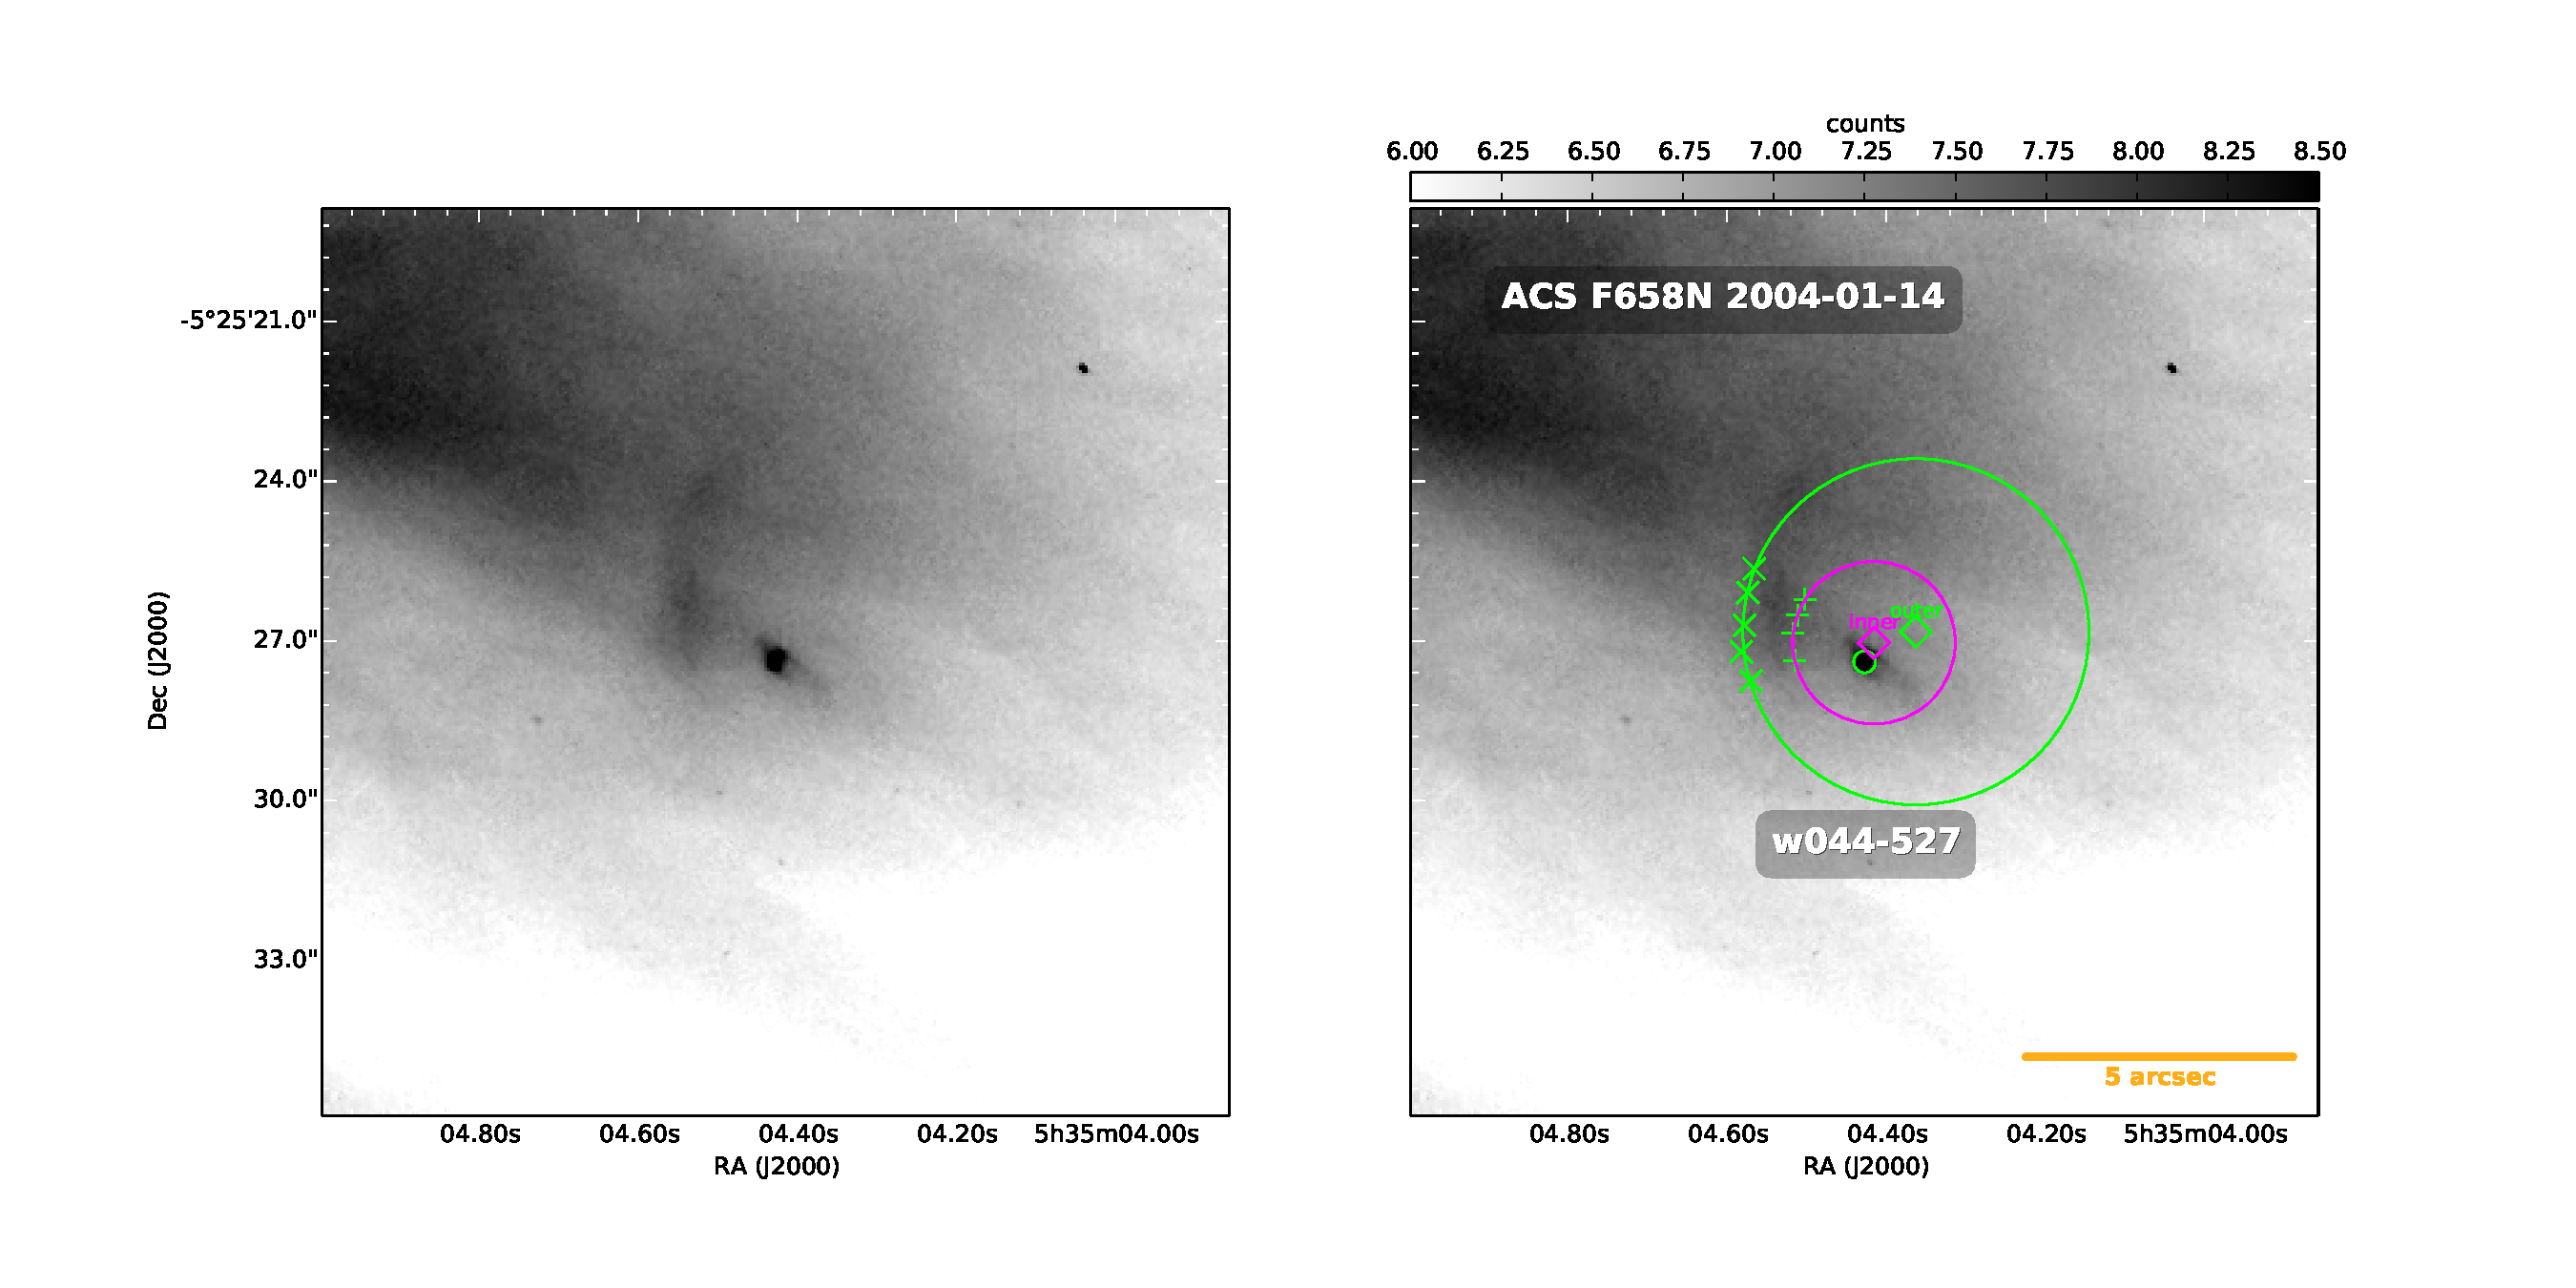
\includegraphics[width=0.5\linewidth, trim=60 50 100 50]{j8oc01010_wcs/w044-527-Bally_01-images.pdf}
    &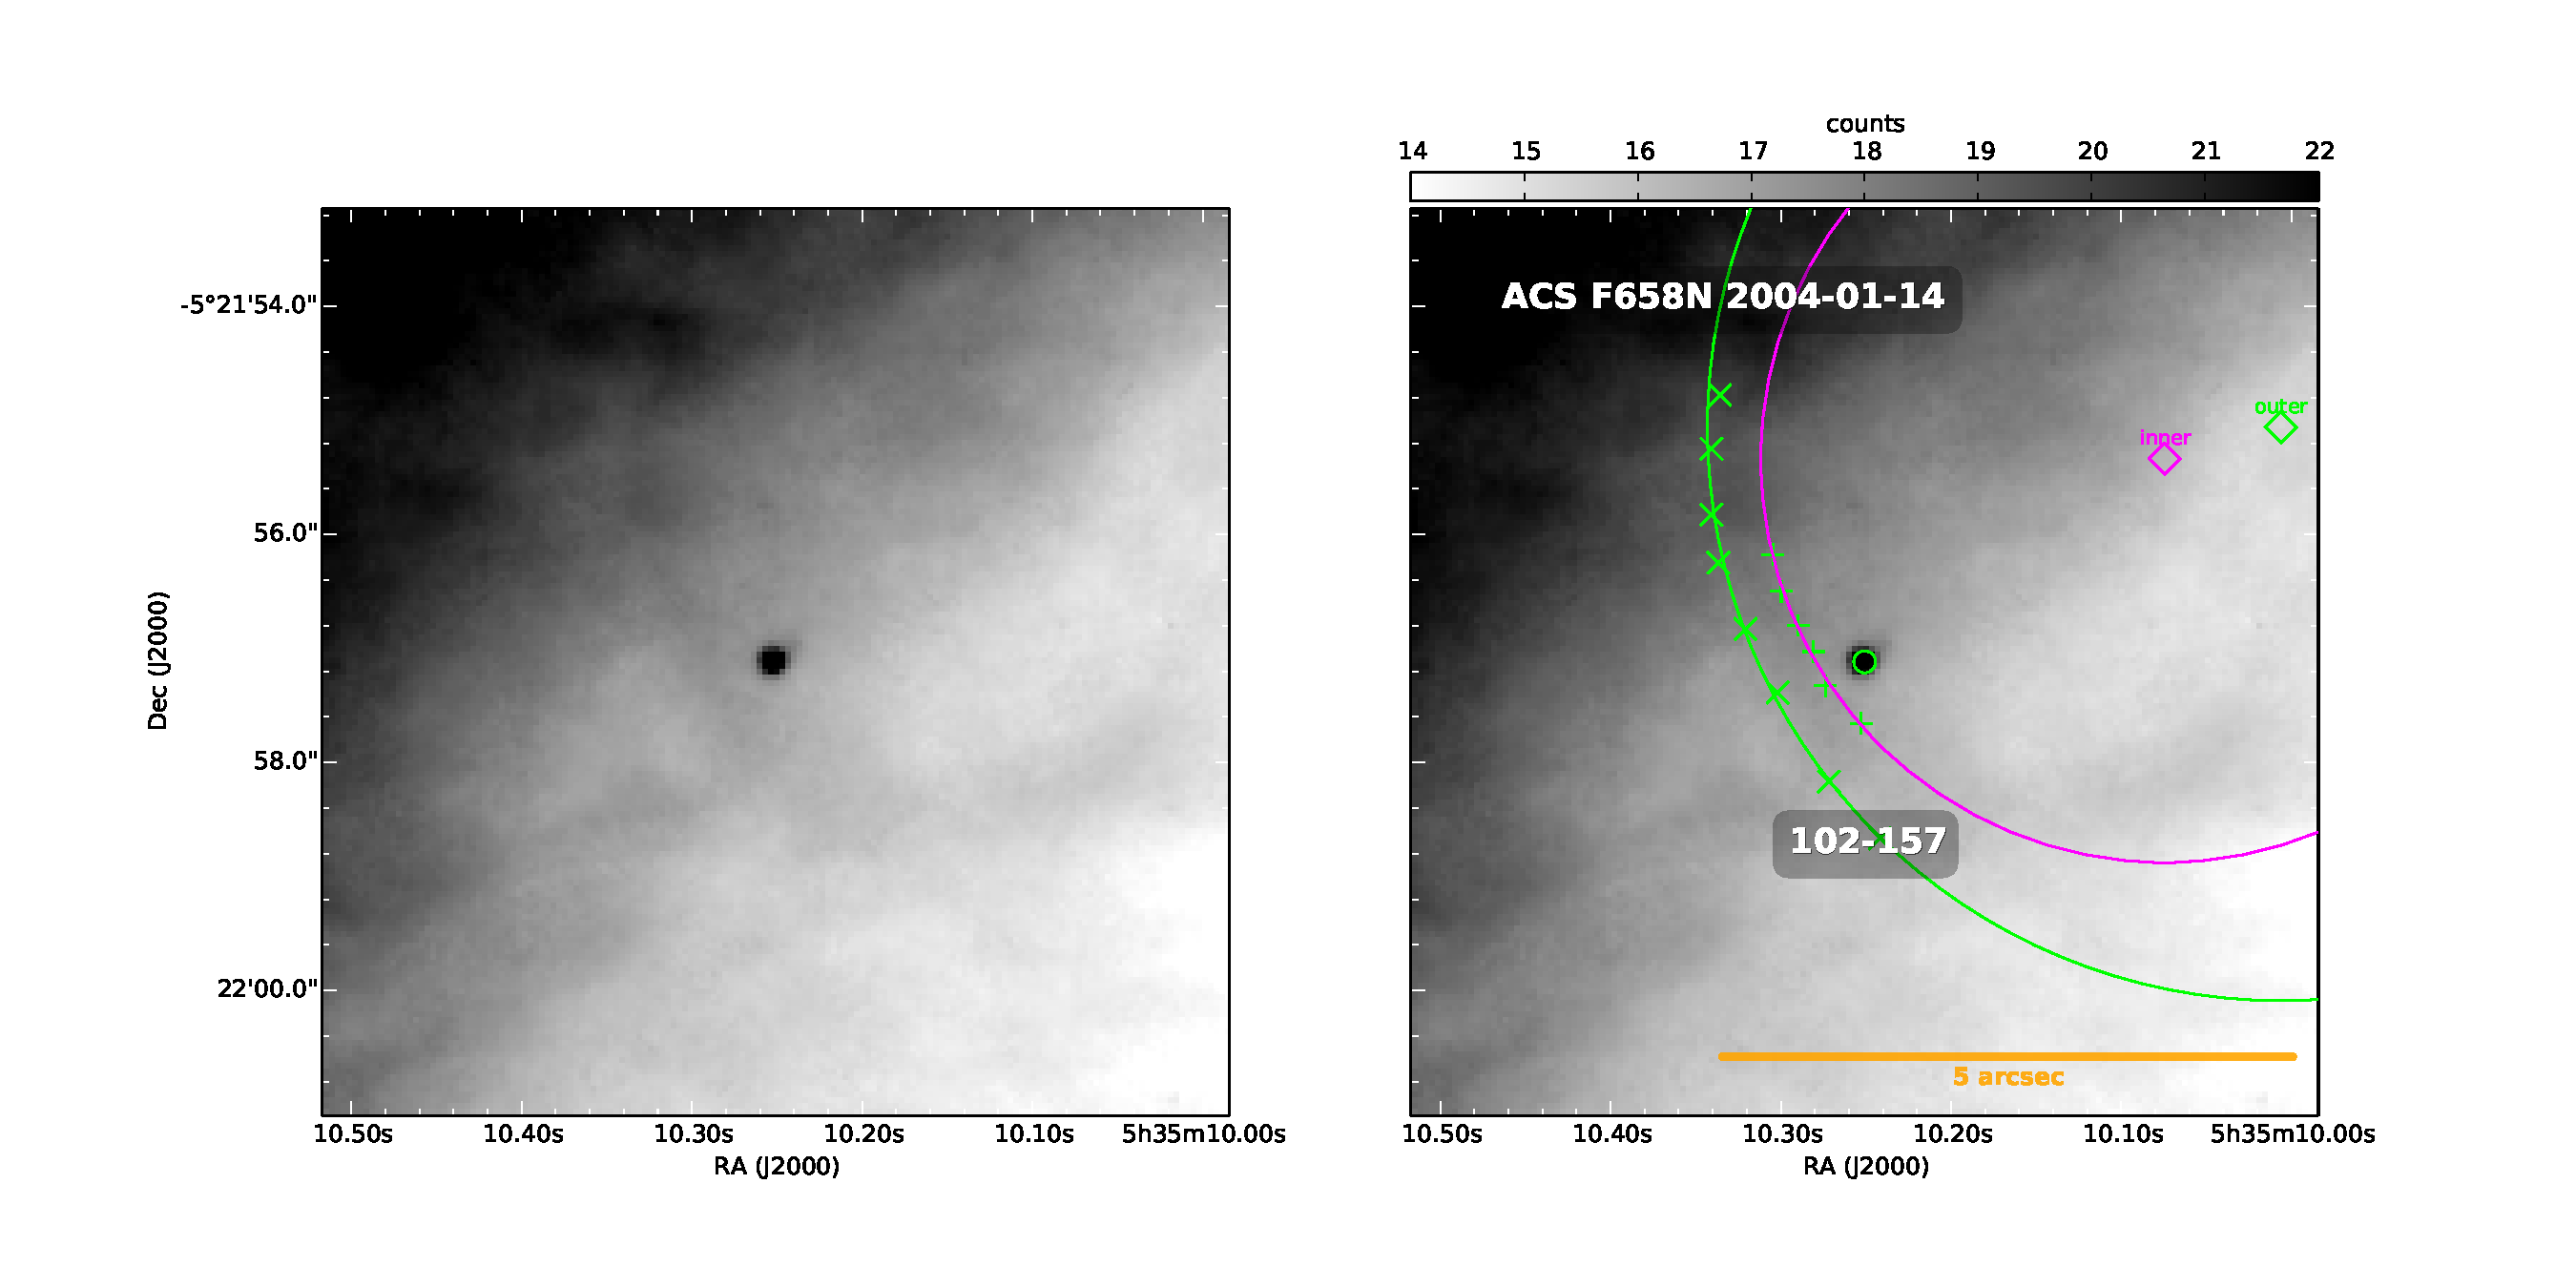
\includegraphics[width=0.5\linewidth, trim=60 50 100 50]{j8oc01010_wcs/102-157-Bally_01-images.pdf}\\
    \includegraphics[width=0.5\linewidth, trim=60 50 100 50]{j8oc06010_wcs/205-230-Bally_06-images.pdf} 
     &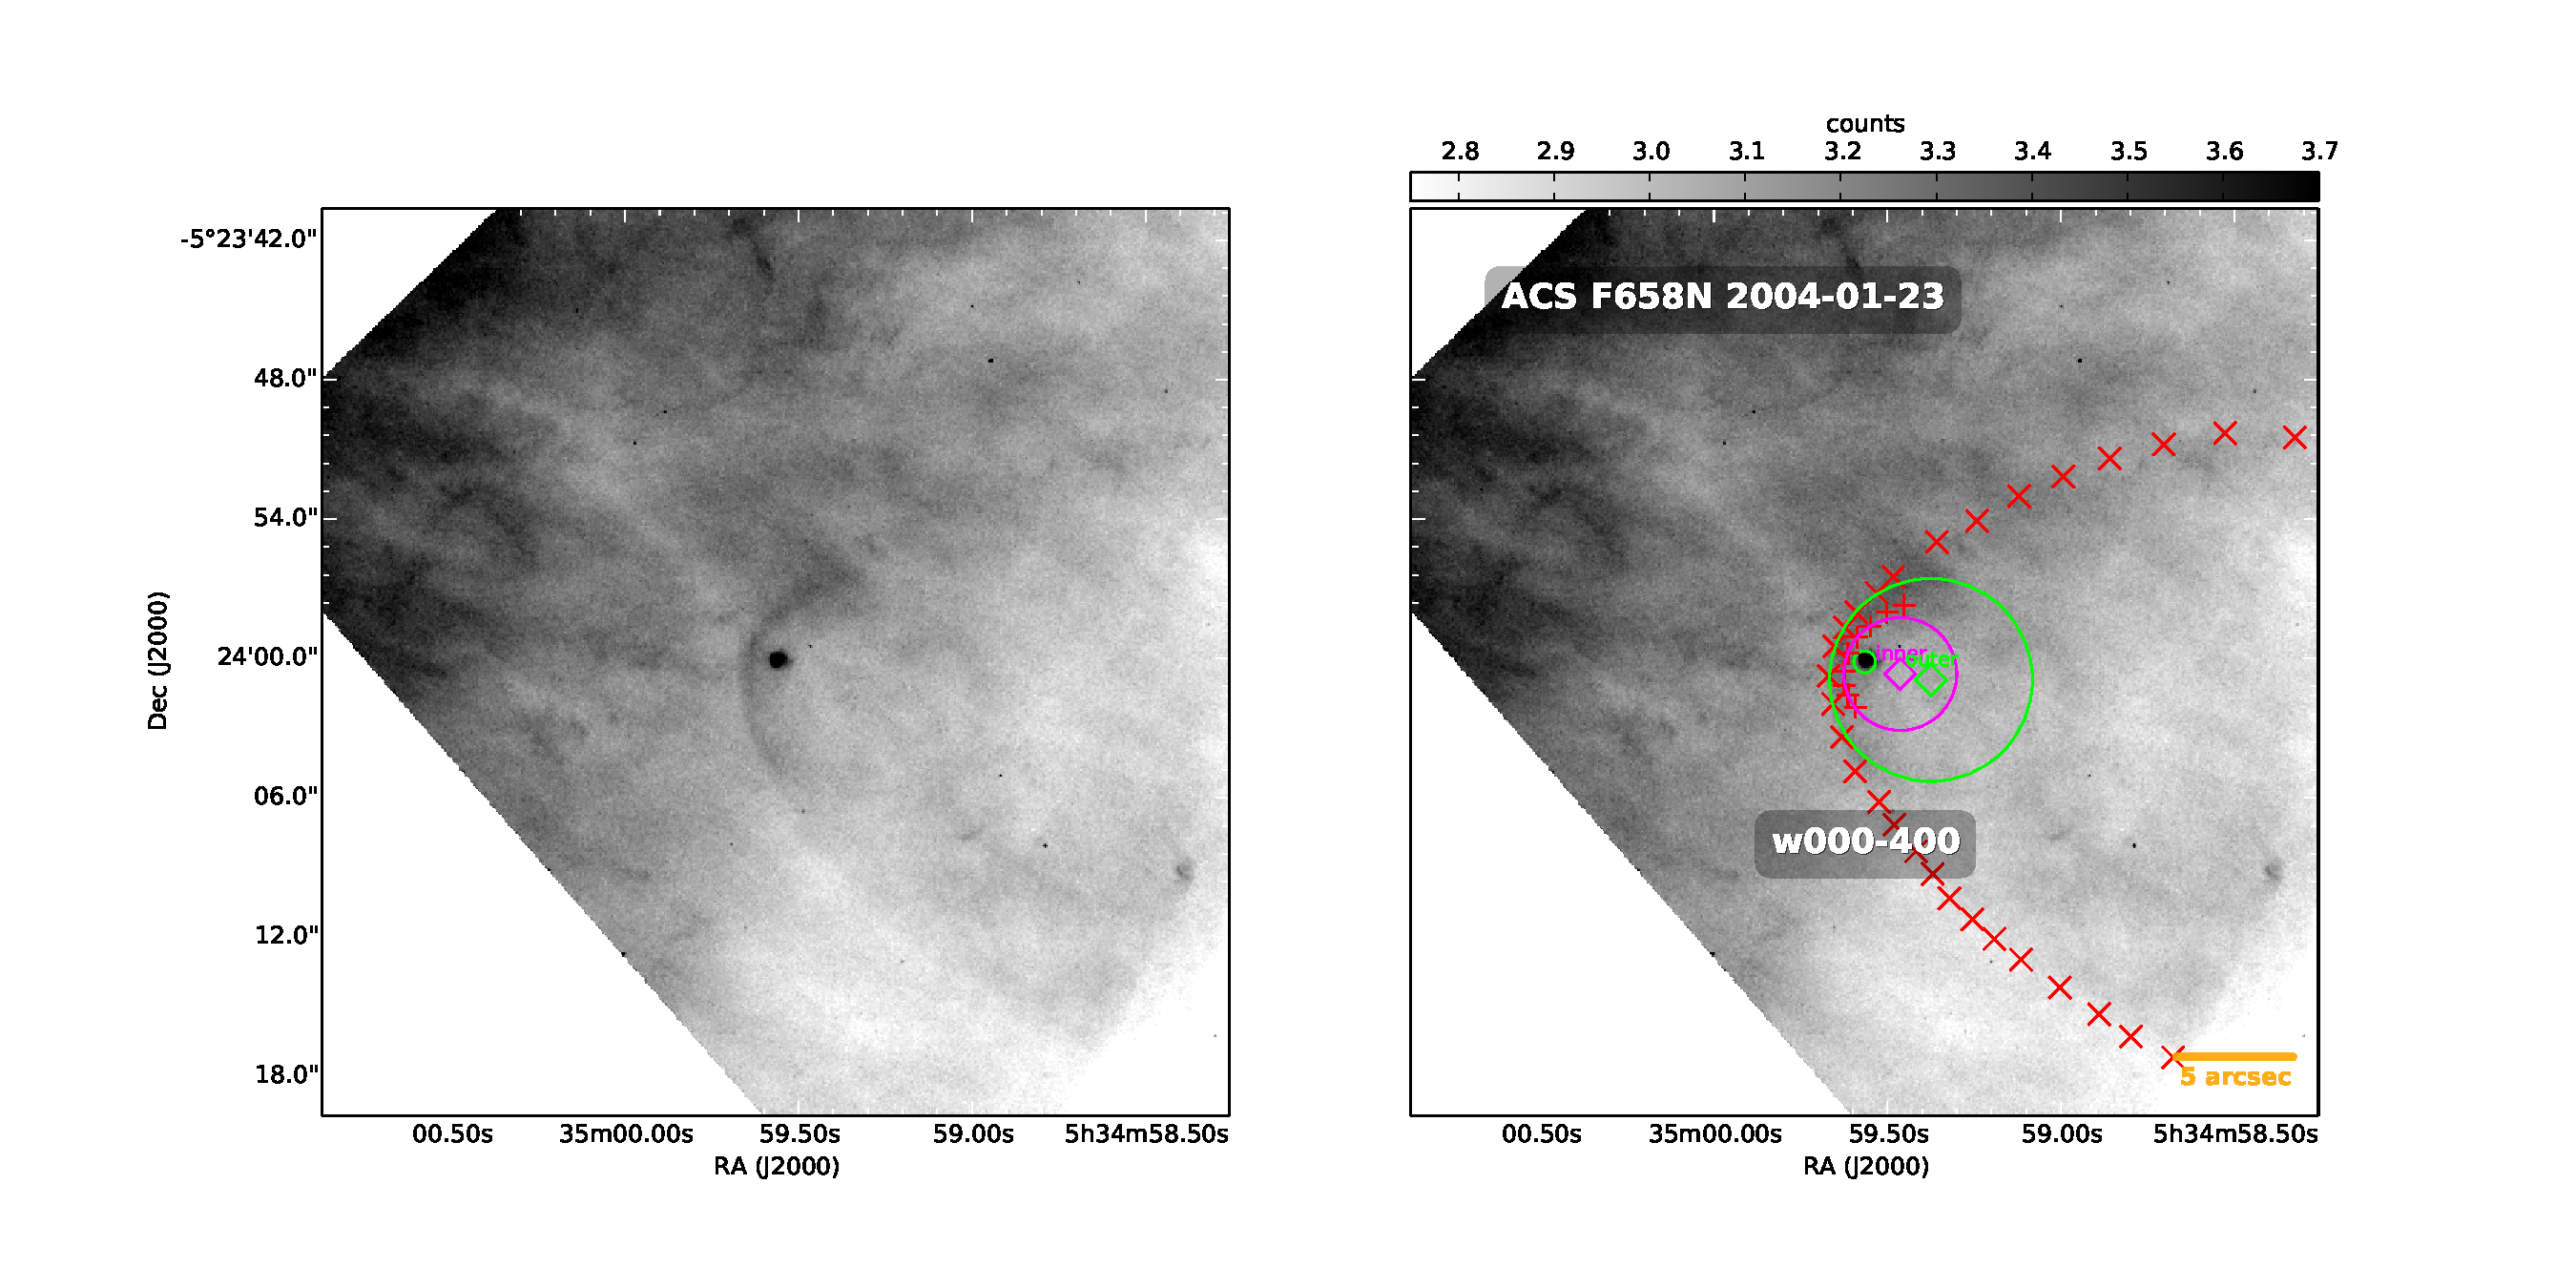
\includegraphics[width=0.5\linewidth, trim=60 50 100 50]{j8oc09010_wcs/w000-400-Bally_09-images.pdf}\\ 
    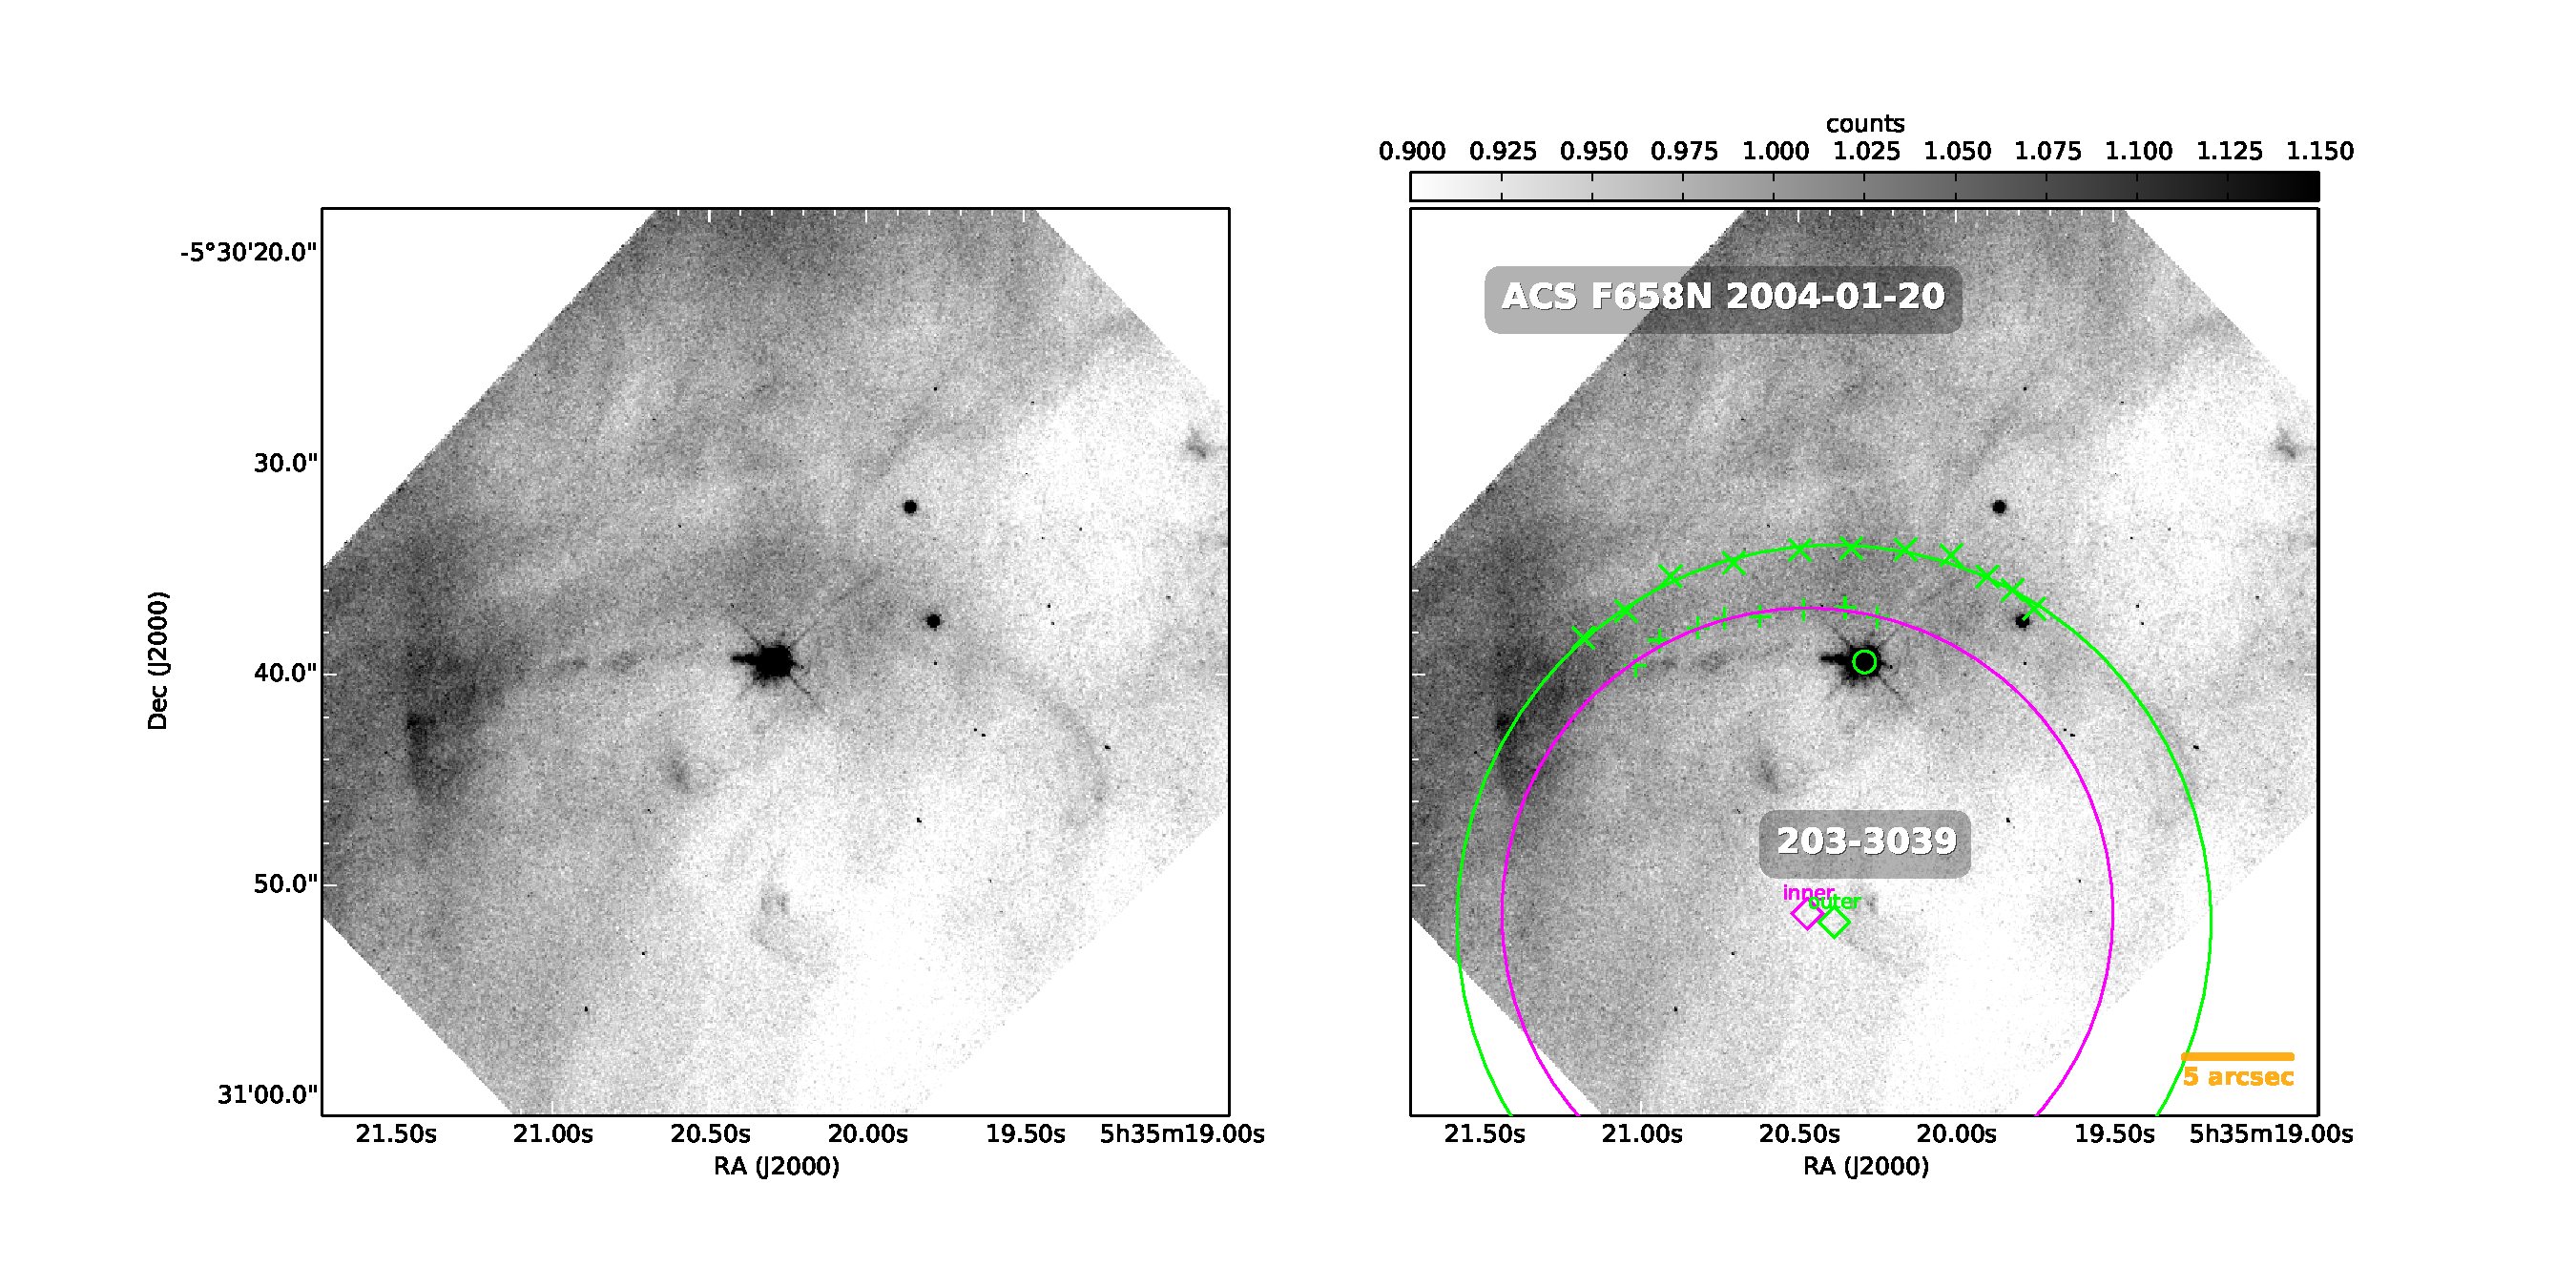
\includegraphics[width=0.5\linewidth, trim=60 50 100 50]{j8oc14010_wcs/203-3039-Bally_14-images.pdf}
    &\includegraphics[width=0.5\linewidth, trim=60 50 100 50]{j8oc16010_wcs/w005-514-Bally_16-images.pdf}\\ 
    \includegraphics[width=0.5\linewidth, trim=60 50 100 50]{j8oc16010_wcs/042-628-Bally_16-images.pdf} 
    &\includegraphics[width=0.5\linewidth, trim=60 50 100 50]{j8oc17010_wcs/LL3-Bally_17-images.pdf}\\ 
    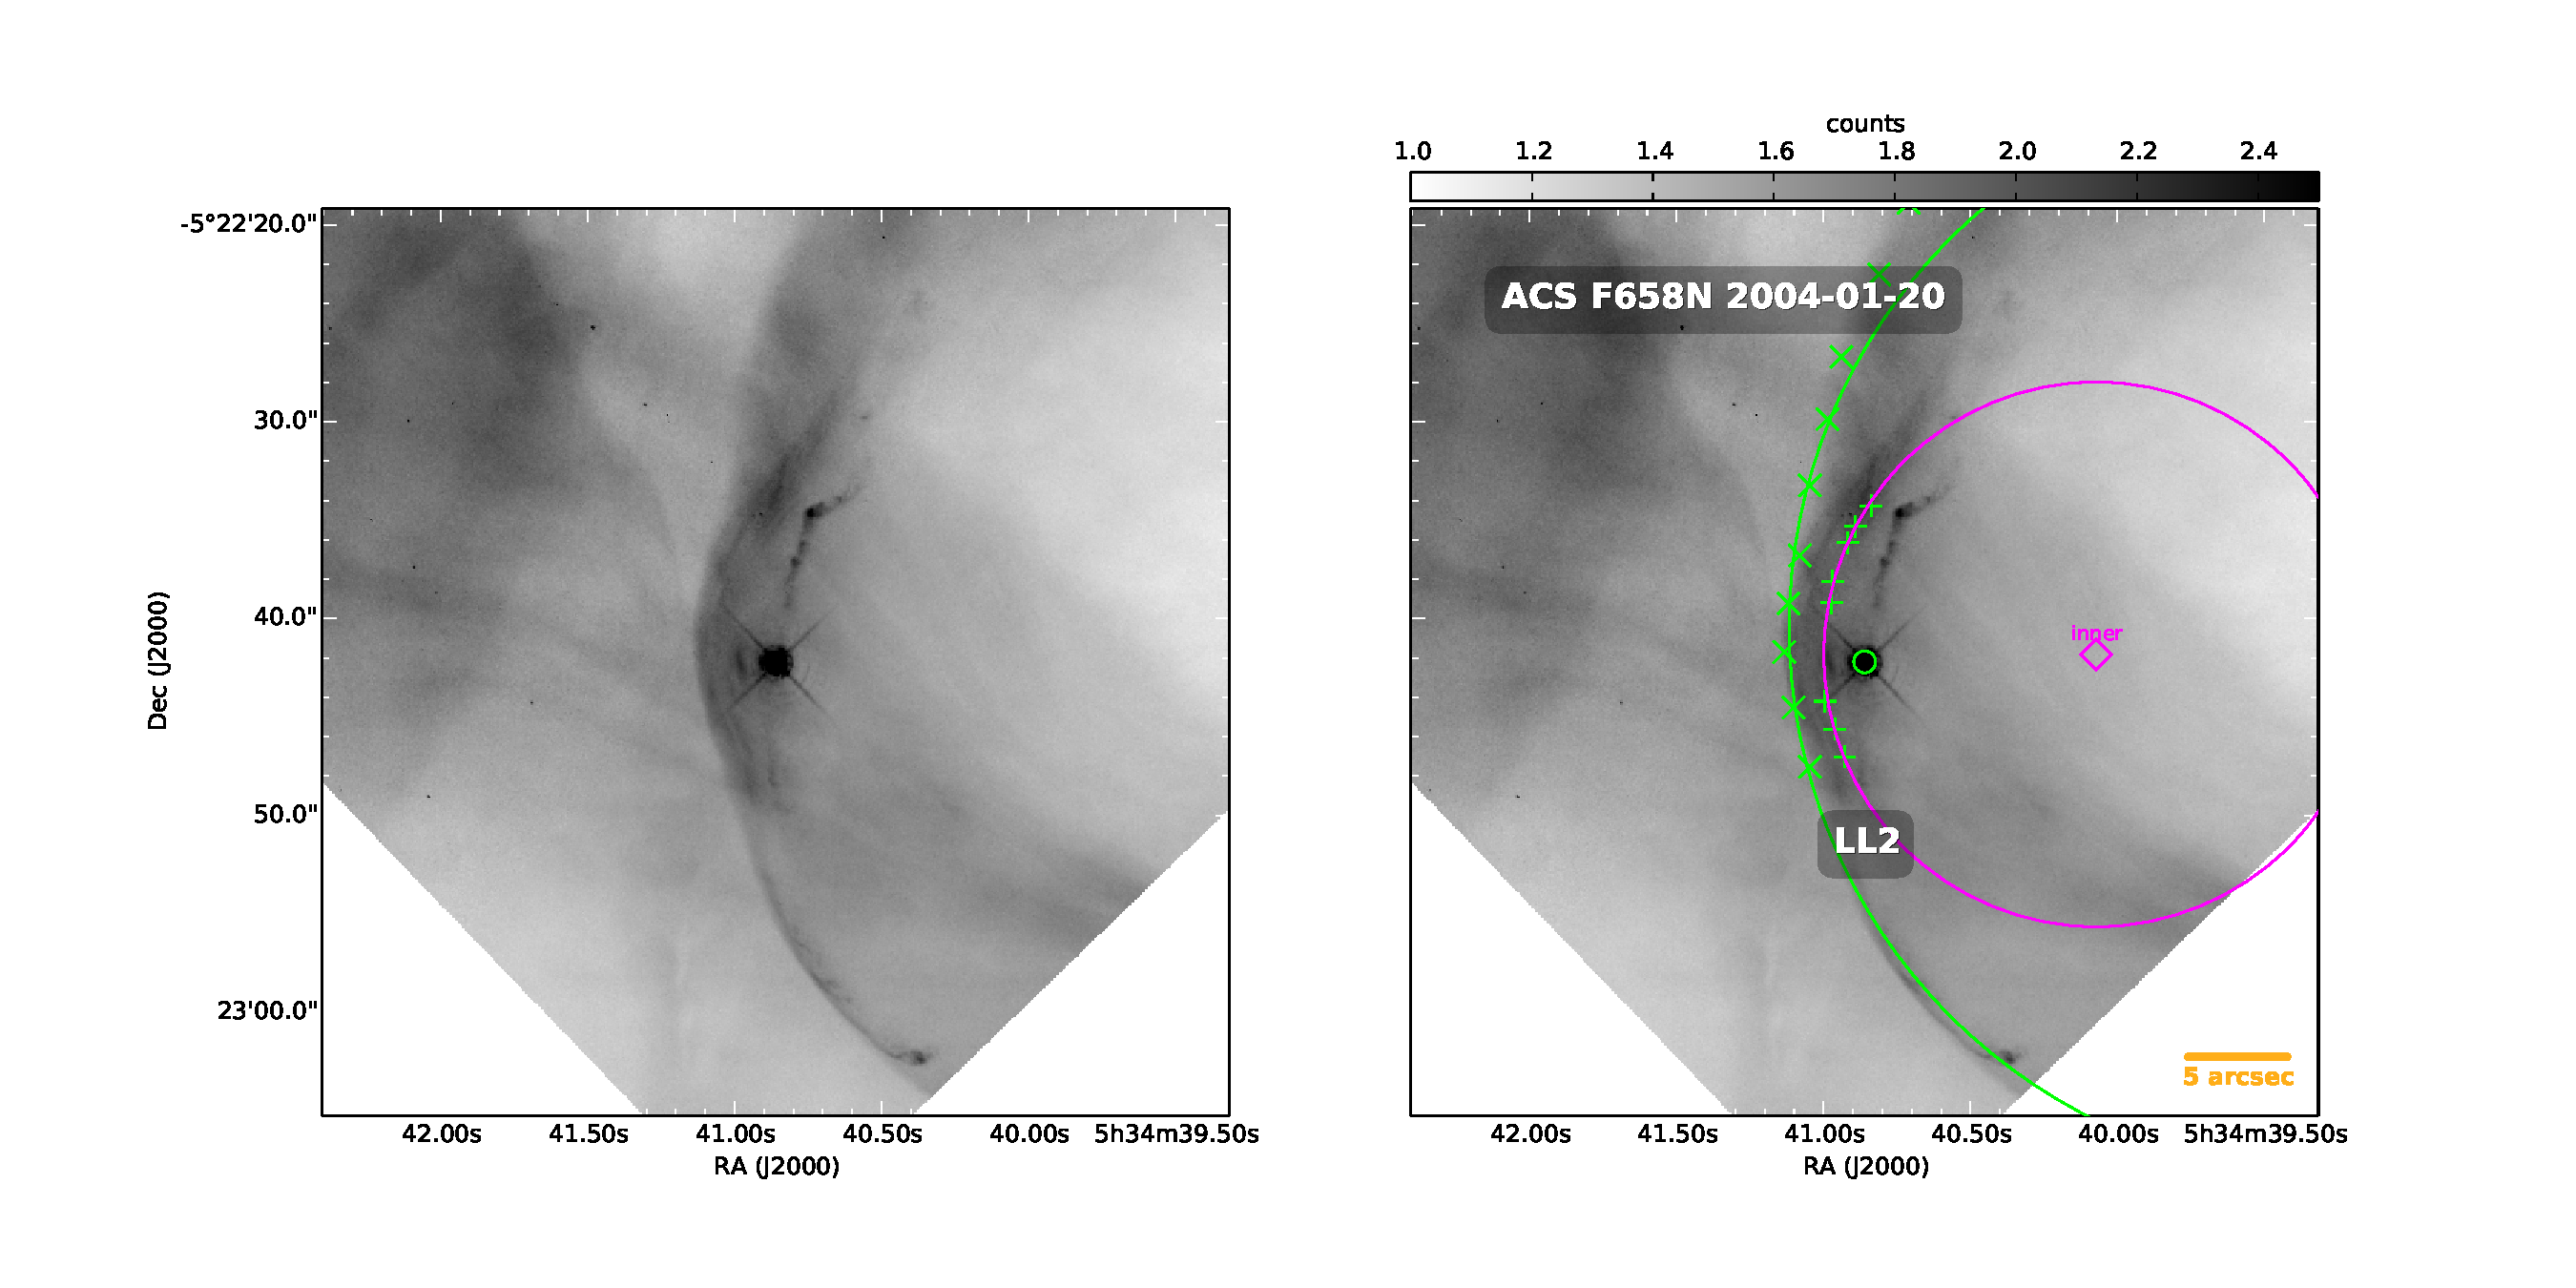
\includegraphics[width=0.5\linewidth, trim=60 50 100 50]{j8oc18010_wcs/LL2-Bally_18-images.pdf}
    &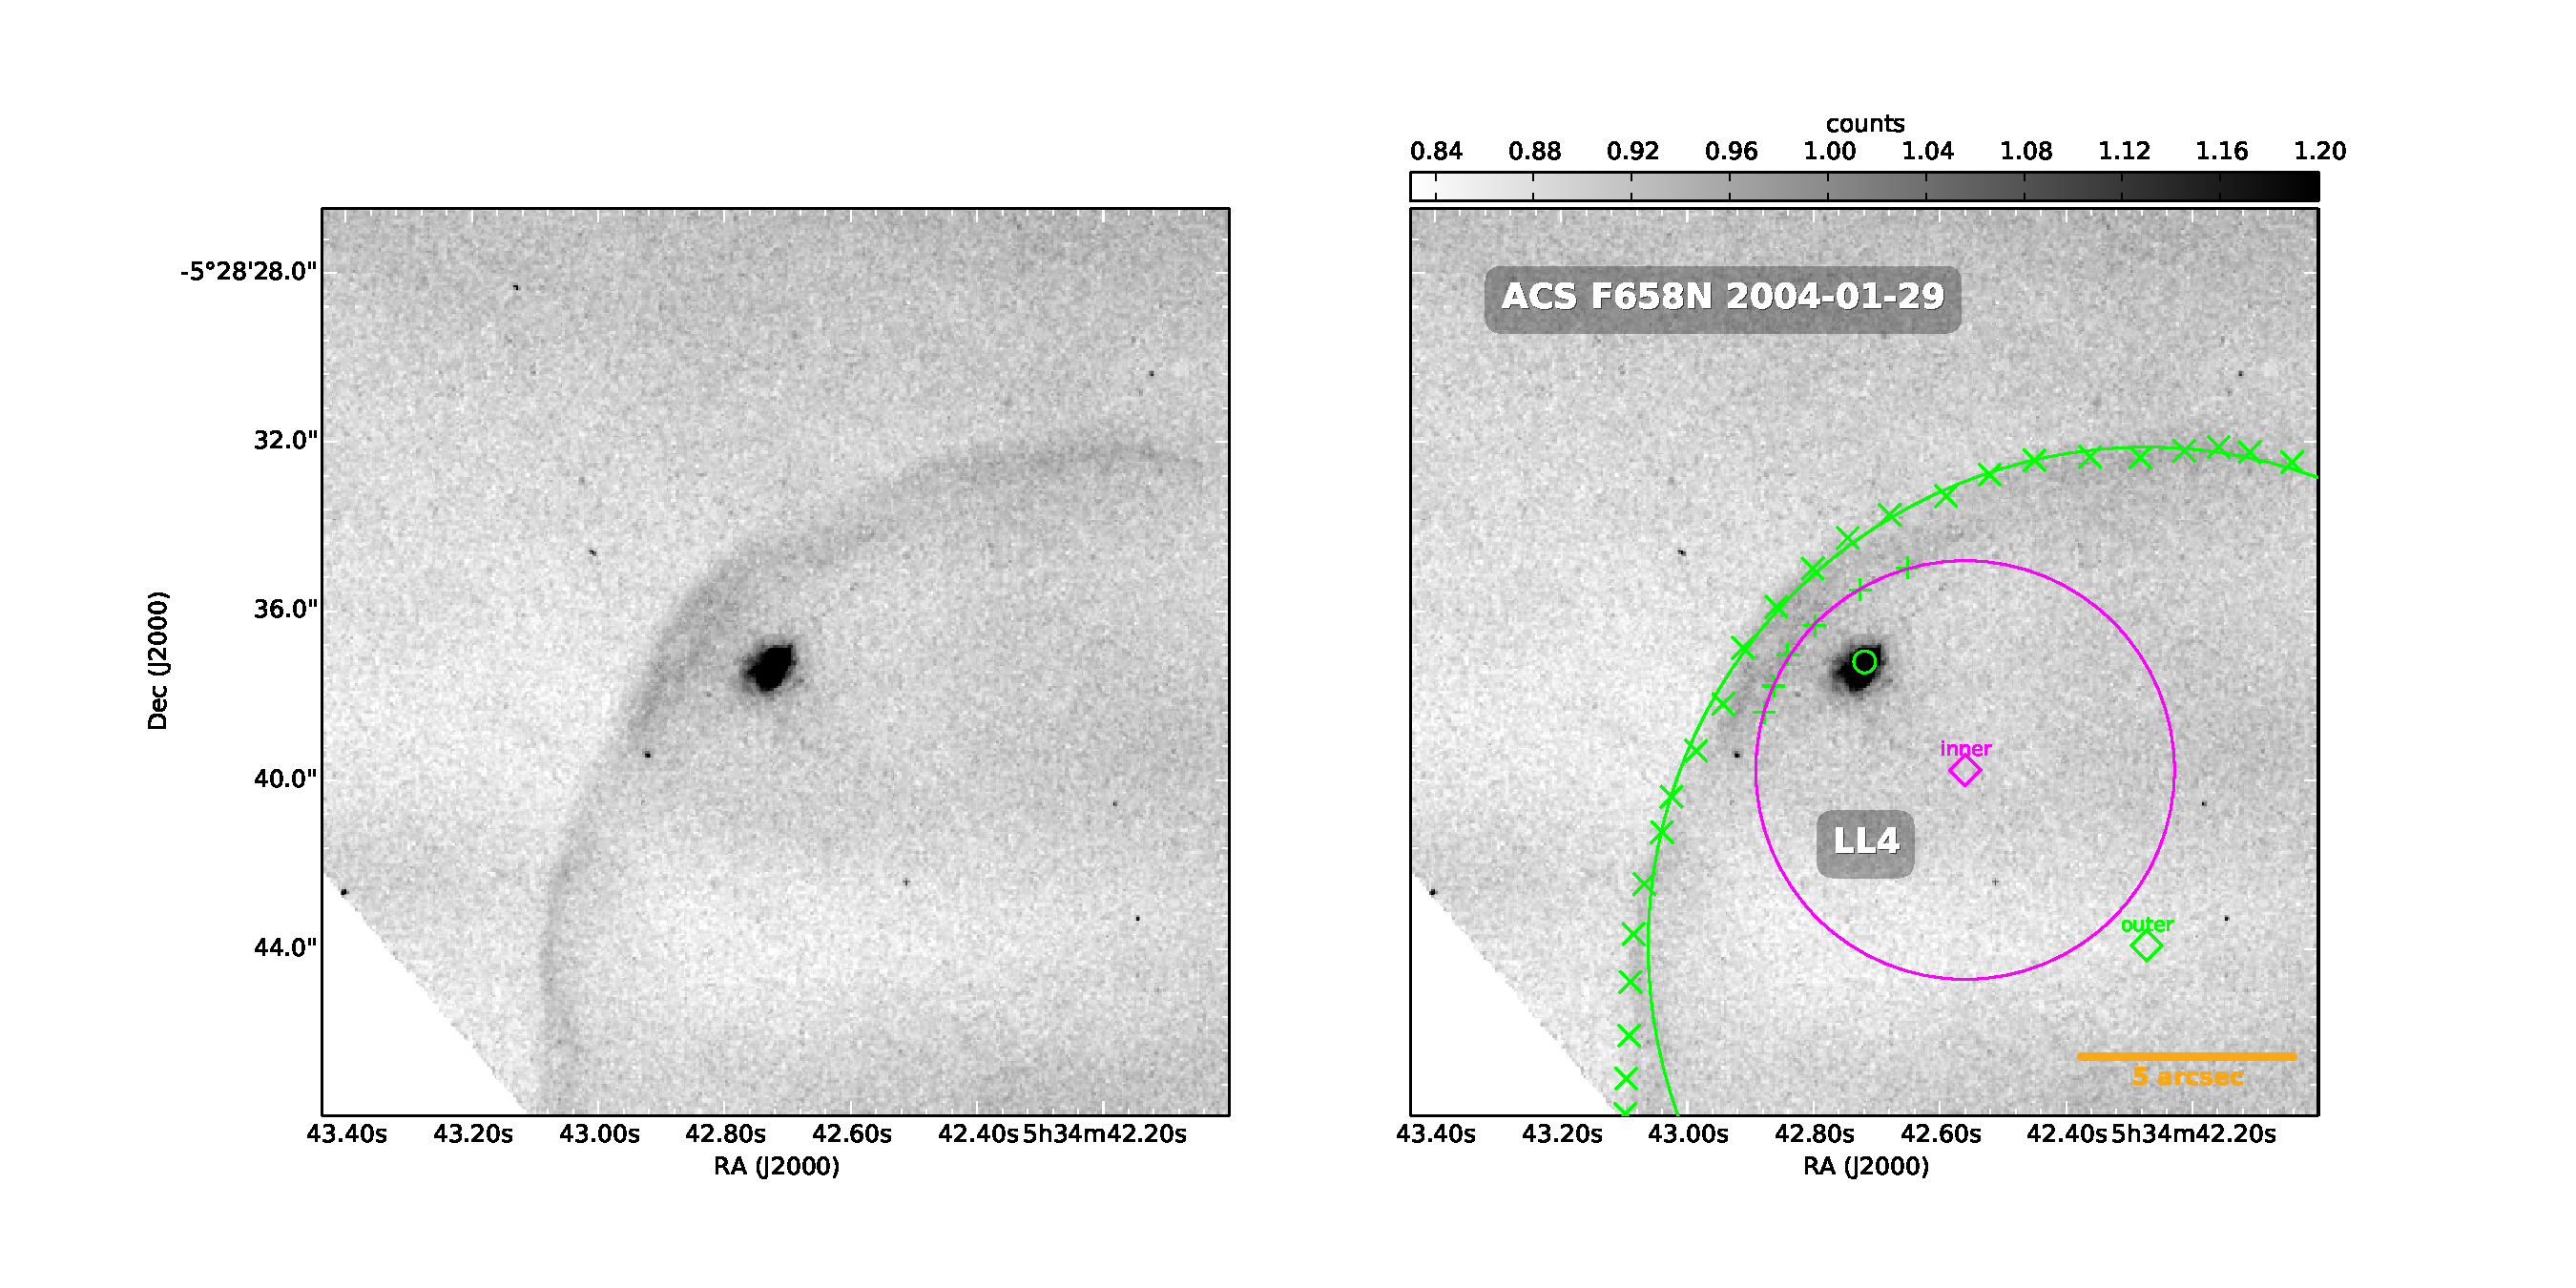
\includegraphics[width=0.5\linewidth, trim=60 50 100 50]{j8oc24010_wcs/LL4-Bally_24-images.pdf}\\
    
\end{tabular}
\end{figure*}

\end{document}